\documentclass[10pt]{article}
\usepackage[margin=.8in]{geometry}\usepackage{amsmath,tikz,hyperref}
\setlength{\parindent}{0pt}\setlength{\parskip}{7pt}
\begin{document}
\textbf{Coefficient array storage correspondence}\hfill2026-10-31\\T-1163. Producer proof; independent source-fidelity review pending.

Bounds-checked array replacement preserves length, writes the selected slot and leaves every other slot unchanged. Canonical residues remain canonical when the replacement is canonical.

For prime $p$ with $1<p<2^{31}$, canonical coefficients and parameters, nonzero scale $s$, and $0\le j\le k\le5$, the composed generated-inverse update gives
\[
 \operatorname{decode}(\mathrm{out}'_i)=\operatorname{decode}(\mathrm{out}_i)+
 \begin{cases}c\binom{k}{j}a^jb^{k-j}s^{-1}&i=j,\\0&i\ne j.\end{cases}
\]
The source index condition $j\le k<\mathrm{length}$ proves the array access is in bounds.
\begin{center}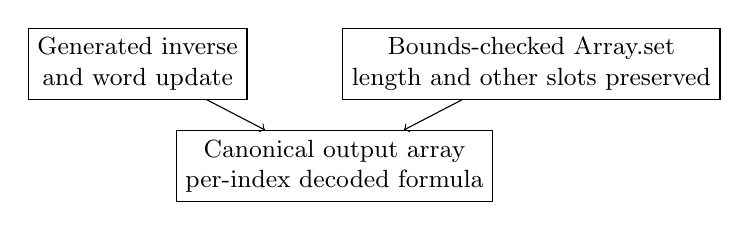
\begin{tikzpicture}[every node/.style={draw,align=center,font=\small}]
\node(a)at(0,0){Generated inverse\\and word update};
\node(b)at(5,0){Bounds-checked Array.set\\length and other slots preserved};
\node(c)at(2.5,-1.3){Canonical output array\\per-index decoded formula};
\draw[->](a)--(c);\draw[->](b)--(c);
\end{tikzpicture}\end{center}
Seven main declarations and eight controls have separate named axiom readbacks. Controls cover first/middle/last replacements, preserved neighbours, empty-array size, an excluded out-of-bounds index, canonical zeros and an actual generated coefficient update. The first attempt needed explicit \texttt{Array.getElem\_set} rewriting for untouched slots; the corrected attempt passed. The first controls attempt needed an explicit three-index split in place of an unavailable tactic. A second controls attempt needed the literal size and proof-dependent hypotheses handled explicitly. All native receipts and warnings remain recorded.

This is one finite-array mutation composed with checked arithmetic. Full nested-loop accumulation, trailing-zero trimming and fixed-size divisor copying remain the next bindings. Lean array semantics are a source storage model, not compiled-Rust equivalence.

Source bindings: \texttt{projective\_law\_gate.rs} transform; preceding \texttt{Loop.lean}, \texttt{WordCoefficient.lean}, \texttt{Inversion.lean}. Primary reference: \href{https://lean-lang.org/doc/api/Init/Data/Array/Set.html}{Lean Array.set semantics}. No novelty claim for standard array or field identities.

Native exit codes, unchanged source/dependency bindings and axiom readback accompany this PDF, editable SVG and structured status. Existing compiled dependencies remain in the trust boundary. No scientific run, timing or cost ratio.
\end{document}
